\subsection{Plotting Multiple Statistical Analyses}
In section \ref{sec:SAraven} we covered how to perform statistical analysis and print the results to an XML
file.  However, what if we want to use the statistics calculated in more RAVEN calculations, like plotting and
further postprocessing?

In the following two sections, we consider two use cases.
\begin{itemize}
  \item In the first case, we want to compare the statistics obtained by three different sampler types on the
    same model. We want to run the sampling, analyze the statistics, then make two plots where we can see how
    the means and variances of the data compare between the sampling strategies.  The plots will have the
    sampler type on the x-axis, and the metric values on the y-axis.
  \item In the second case, we want to see the time evolution of the statistics; that is, the mean and 5/95
    percentile of the model output as it evolves in time.  We want to plot this so that the x-axis is time,
    and the y-axis is the model output value, with three series, one each for fifth percentile, mean, and
    ninety-fifth percentile.
\end{itemize}

Note that while we use the `BasicStatistics` postprocessor as an example, there are many other RAVEN
postprocessors that produce XML outputs that follow this same strategy.

\subsubsection{Case 1: Comparing Samplers}
In this case, we are interested in comparing the statistics obtained by several samplers (Monte Carlo, Grid,
and Stratified/Latin Hypercube) on a plot.  To do
this, we need to complete the following steps:
\begin{enumerate}
  \item Sample the model using Monte Carlo, Grid, and Stratified samplers, storing results in separate point
    sets.
  \item Perform statistical analysis (mean and variance) on each of the point sets containing the samples, writing results to
    separate RAVEN XML output files.
  \item Read in the RAVEN XML output files, creating a point set with the sampler types as inputs and the mean
    and variance as outputs.
  \item Plot the metrics as a function of the sampler used.
\end{enumerate}

These steps lead to the following \xmlNode{RunInfo} block, see especially the \xmlNode{Sequence}:
\xmlExample{framework/user_guide/StatisticalAnalysis/comparingSamplers.xml}{RunInfo}
Note that each sampling and statistics requires its own step, which grows our total steps from four
conceptually to eight in RAVEN.

Next, let's define the \xmlNode{Steps} block that will execute this \xmlNode{sequence}:
\xmlExample{framework/user_guide/StatisticalAnalysis/comparingSamplers.xml}{Steps}

The three ``sample'' steps take the code input (\xmlString{referenceInput}) as input, define the code itself
(\xmlString{bateman}), indicated the sampler to use in each, and then output the results to a
\xmlNode{PointSet}.

The three ``stats'' steps take one of the point sets as input, use the basic statistics postprocessor as the
model, and output to a RAVEN XML output file.  Note that we can re-use a single basic statistics
postprocessor, rather than create separate entities.

In the \xmlString{readStats} step, the three RAVEN XML output files are inputs to the RavenOutput
postprocessor model, and result in a \xmlNode{PointSet} that has the statistics from each file in a single
data object.

In the \xmlString{plot} step, the statistics data object is passed to two \xmlNode{OutStream} plotters.  We
include the \xmlAttr{pauseAtEnd} attribute to ensure plots printed to screen are retained.

With the \xmlNode{Steps} defined, we now define all the entities used throughout the calculation.  We won't go
over them in great detail, but will point out a few notable features:
\begin{itemize}
  \item Data Objects:
    \begin{itemize}
      \item There are three data objects for storing the samples from the samplers, and one to hold the
        statistics.  Note that while the output of the Bateman code is histories, since we only define
        \xmlNode{PointSets} the code keeps only the final value for output values.
    \end{itemize}
  \item Files:
    \begin{itemize}
      \item In order for RAVEN to keep track of the XML files in which the statistics will be written, we
        define them in the \xmlNode{Files} block.  Note that these files need not exist before the RAVEN run
        starts; they will be created in the run.
      \item Additionally, we define the input template for the code itself, used in all the sampling steps.
    \end{itemize}
  \item Models:
    \begin{itemize}
      \item In the Models we define the interface to the Bateman code as well as the two postprocessors.
      \item Note that in the \xmlNode{BasicStatistics} we request the expectedValue, variance, and number of samples as
        metrics for all four outputs of the Bateman model, even though we only need the expectedValue and
        variance for output C.  This demonstrates the ability of the RavenOutput postprocessor to be selective
        about the values it retains.
      \item In the \xmlNode{RavenOutput} postprocessor, there are two operation modes, \xmlNode{dynamic} and
        non-dynamic.  Because the \xmlNode{dynamic} is not specified, we are operating in static mode (we look
        at dynamic mode in the next section).  This means we specify several files to load from.  Ultimately
        we want a point set that contains the following information:
        \begin{center}
        \begin{tabular}{c | c | c }
          ID & mean & variance \\ \hline
          1 & MC mean & MC variance \\
          2 & Grid mean & Grid variance \\
          3 & LHS mean & LHS variance
        \end{tabular}
        \end{center}
        To get these values, we assign a float file ID to each file in the \xmlAttr{ID} attribute.  These
        values can be whatever we want; they'll be used to keep track of which set of outputs come from which
        sampling strategy.  Within the \xmlNode{Files} node, we instruct the RAVEN XML output reader how to
        read in values using the \xmlNode{output} nodes.  The \xmlAttr{name} attribute determines what column
        (or variable) in the PointSet a value will go in, and the text of the node gives a path in the XML to
        find the value.  For example, \xmlString{C|variance} instructs the postprocessor to look in the RAVEN
        XML output file under the node \xmlNode{C} for a node named \xmlNode{expectedValue}, and use its
        value.

        Over the process of reading all the files, entries for both the mean and variance are collected,
        giving us a data set of realizations where the input space is the file ID and the output space are the
        desired metrics.  Note that it is not necessary to retain the original name of the statistics; we
        chose the shorter name ``mean'' to read in the ``expectedValue'' entries.
    \end{itemize}
  \item Samplers and Distributions:
    \begin{itemize}
      \item The Distributions are unchanged from previous examples.
      \item In defining the three samplers, we only note that we specified the number of samples so that they
        were equivalent across all three samplers in an effort to make a fair comparison.
    \end{itemize}
  \item OutStreams:
    \begin{itemize}
      \item We define our two plots here, using fairly standard syntax.  Note that when these plots are
        generated, the File IDs are on the x-axis, while the statistics metric (mean or variance) values are
        on the y-axis.  The File IDs can be traced back to the IDs given in the definition of the
        \xmlNode{RavenOutput} postprocessor.
    \end{itemize}
\end{itemize}
When this code is run, the following plots are produced:
\begin{figure}[h!]
  \centering
  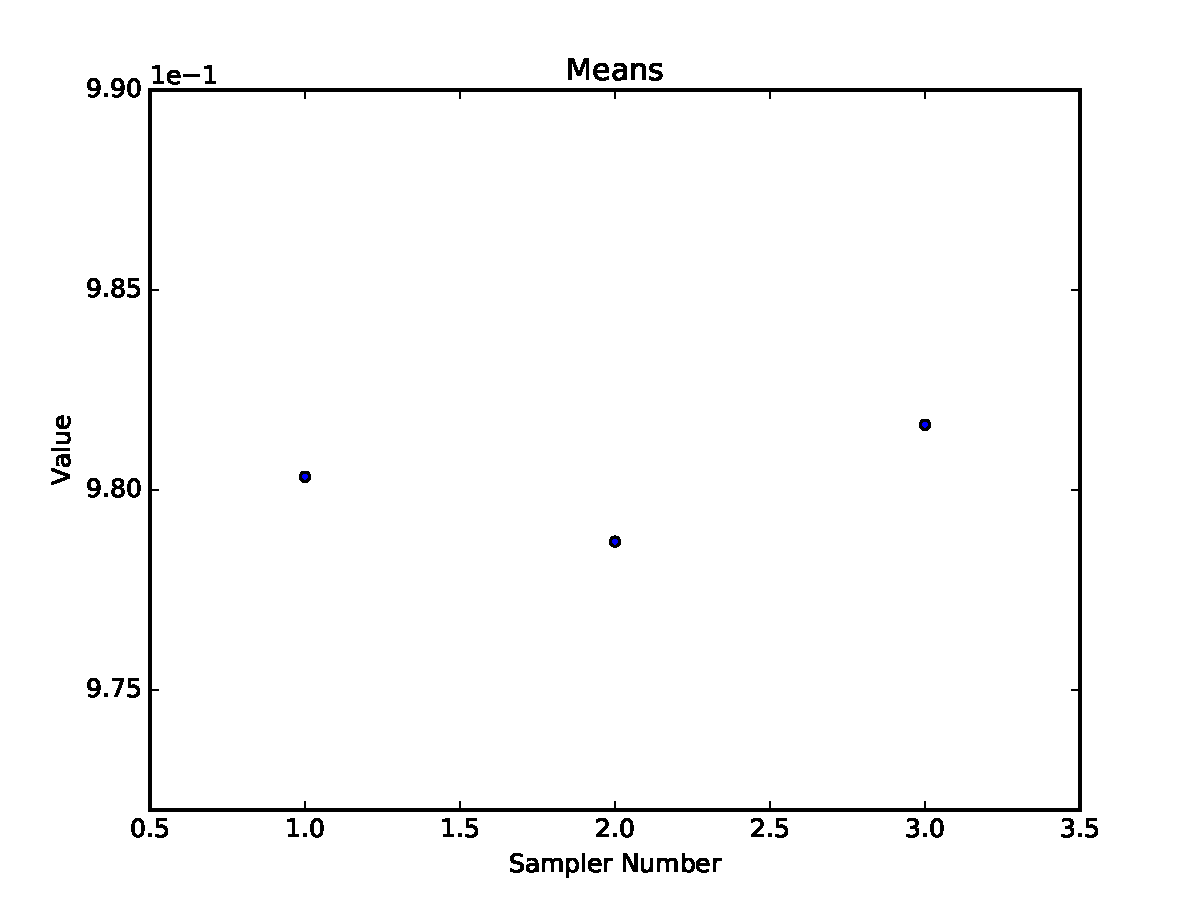
\includegraphics[width=0.7\linewidth]{../../tests/framework/user_guide/StatisticalAnalysis/comparingSamplers/meanPlotter_scatter}
  \caption{Sampler Comparison Plot, Means}
\end{figure}
\begin{figure}[h!]
  \centering
  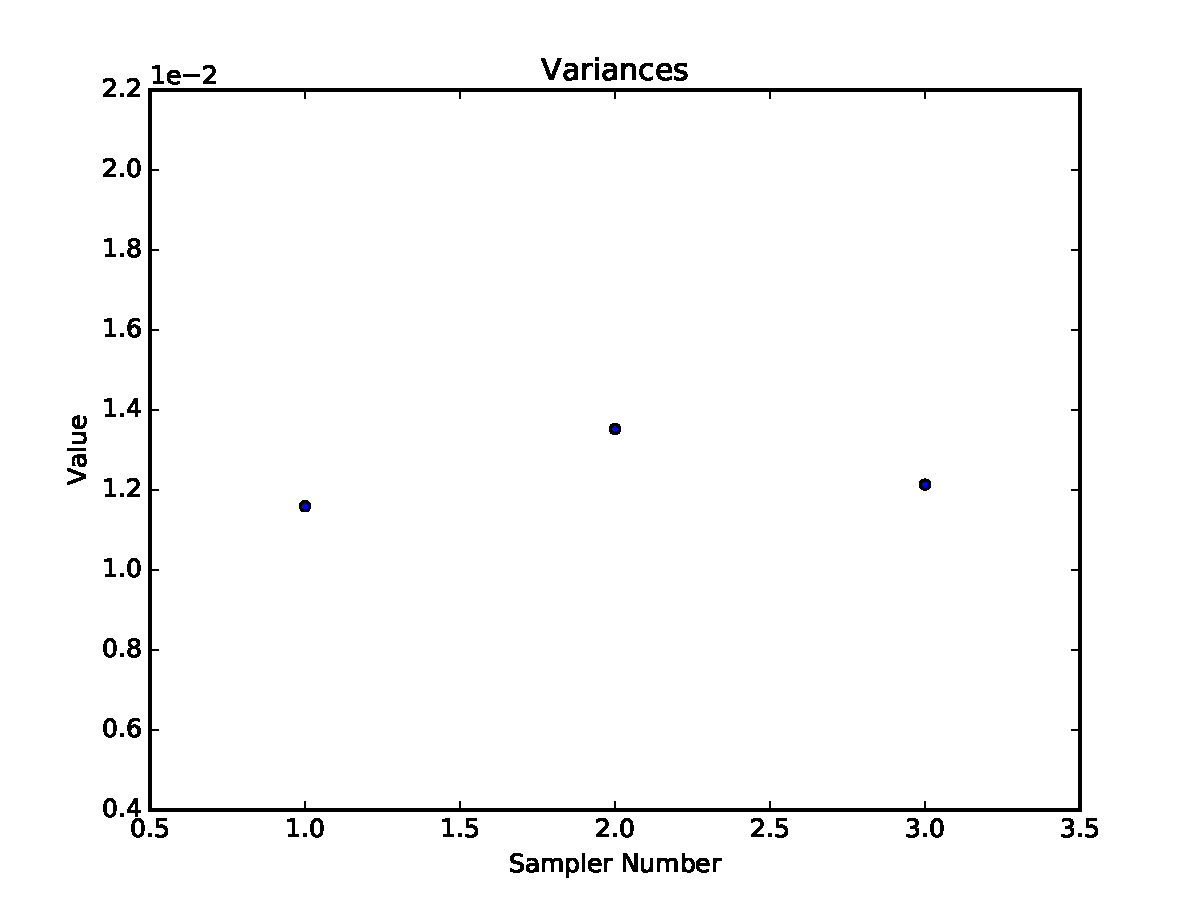
\includegraphics[width=0.7\linewidth]{../../tests/framework/user_guide/StatisticalAnalysis/comparingSamplers/varPlotter_scatter}
  \caption{Sampler Comparison Plot, Variance}
\end{figure}

